\documentclass{article}
\usepackage{graphicx} % Required for inserting images

\title{Labwork 2: Linear Regression}
\author{Phi Doan Minh Luong - 24400464}
\date{April 2025}

\begin{document}

\maketitle

\setlength\parindent{0pt}

\section{Implementation}
- First, we implement functions to calculate the single loss value, 2 partial derivatives over $w_0$ and $w_1$, and a function to calculate the loss of all data points.

- Read the csv file and extract the value of x and y as lists of floats

- Perform gradient descent to optimize the weights $w_0$ and $w_1$. It iteratively updates $w_0$ and $w_1$ using the gradients (df0 and df1) and the learning rate $lr$

- After training, the optimized weights w0 and w1 are used to plot the regression line based on the learned weights and a plot shows the loss over iterations

- Here is the result when the gradient descent is run for 200,000 iterations with a learning rate of 0.0001 when the initial value for $w_0$ and $w_1$ is 1 and 1 respectively

\begin{center}
    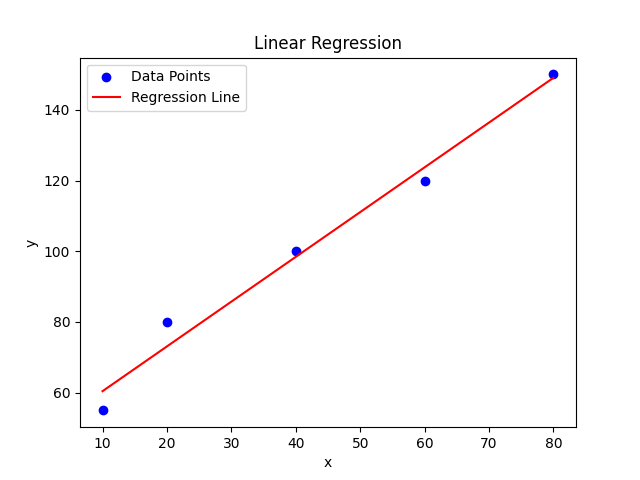
\includegraphics[width=0.5\linewidth]{1.png}

    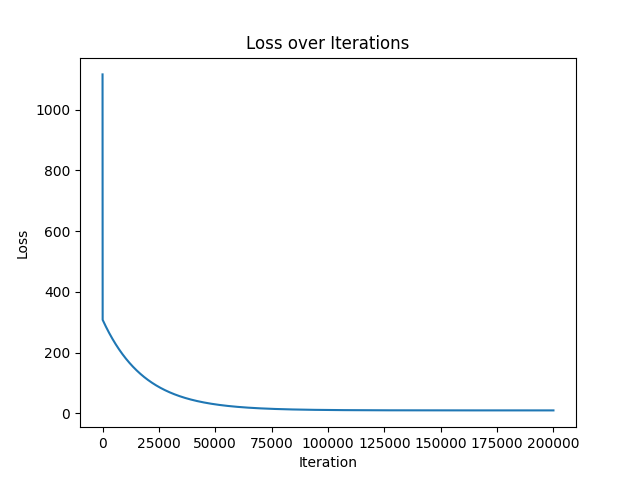
\includegraphics[width=0.5\linewidth]{2.png}
    
\end{center}

- After updating, the loss is around 9.46

\section{The effect of different learning rates for convergence}
\subsection{Learning rate is too small}
- When the learning rate is too small, it requires many updates before reaching
the minimum point
\begin{center}
    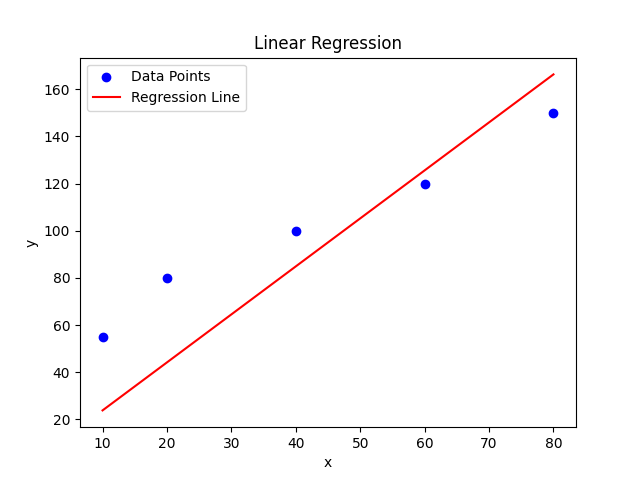
\includegraphics[width=0.5\linewidth]{3.png}

    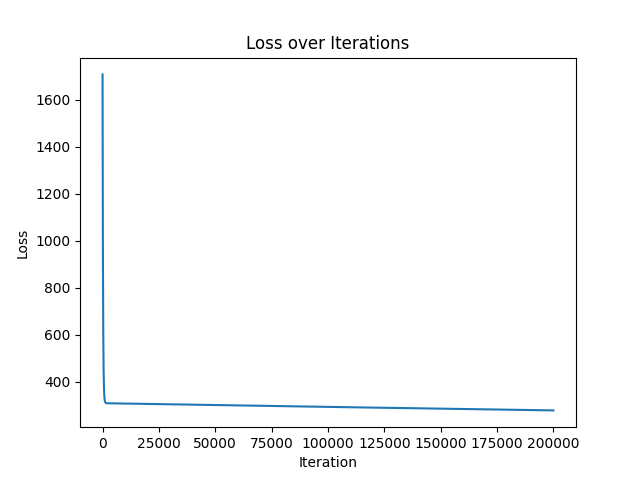
\includegraphics[width=0.5\linewidth]{4.png}
\end{center}

- After updating for 200,000 times, the loss is around 277.74

\subsection{Learning rate is too large}
- When the learning rate is too large, it could cause drastic updates, which lead
to divergent behaviors
\begin{center}
    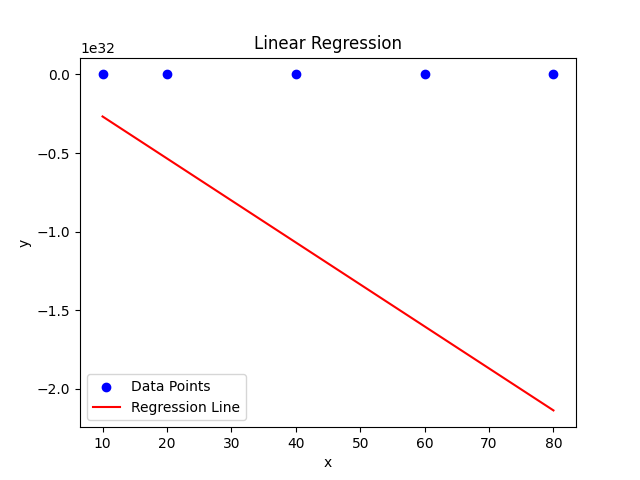
\includegraphics[width=0.5\linewidth]{5.png}

    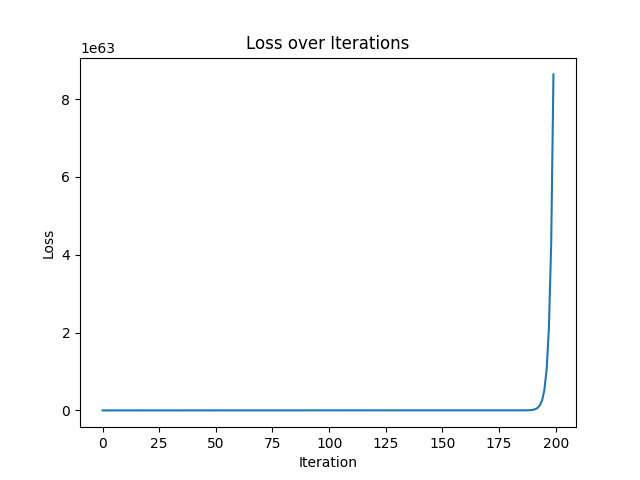
\includegraphics[width=0.5\linewidth]{6.png}
\end{center}

- The algorithm overshoot the minimum and lead to divergence
\end{document}
